\documentclass[portrait]{tikzposter}

%TODO: nullfont ?  Dès le début de l'usage de tikzposter !
%TODO: various font subst to investigate

%\usepackage{type1cm}
\usepackage{pgfplots}
\usepackage{tkz-euclide}% for geometry
\usepackage{tikz-qtree}
\usepackage{lipsum}% for dummy text
\usepackage{multicol}% for multiple columns
\setlength{\columnsep}{4cm}
\setlength{\columnseprule}{1mm}
\usepackage{amsmath}

\definelayouttheme{MyBoard}{
    \usecolorstyle[colorPalette=BlueGrayOrange]{Spain}
    \usebackgroundstyle{Default}
    \usetitlestyle{Default}
    \useblockstyle{Basic}
    \useinnerblockstyle{Envelope}
    \usenotestyle{Sticky}
}

\usetheme{MyBoard}
\colorlet{backgroundcolor}{white}

\pgfplotsset{compat=1.18}

\usetikzlibrary{lindenmayersystems,shadings}% gives us fractals
%\pgfdeclarelindenmayersystem{Koch curve}{
%  \rule{F -> F-F++F-F}}
%\pgfdeclarelindenmayersystem{Sierpinski triangle}{
%  \rule{F -> G-F-G}
%  \rule{G -> F+G+F}}
%\pgfdeclarelindenmayersystem{Fractal plant}{
%  \rule{X -> F-[[X]+X]+F[+FX]-X}
%  \rule{F -> FF}}
%\pgfdeclarelindenmayersystem{Hilbert curve}{
%  \rule{L -> +RF-LFL-FR+}
%  \rule{R -> -LF+RFR+FL-}}

\title{\huge Some Curious Recursive Functions : Hostadter's G and After}
\author{Pierre Letouzey (équipe ACS, ...)}
\institute{IRIF, Université Paris Cité / Picube, INRIA / CNRS}

%% Insert logos to the left and right of tkizposter title
%% Source: StackOverflow

\makeatletter
\newcommand\insertlogoi[2][]{\def\@insertlogoi{\includegraphics[#1]{#2}}}
\newcommand\insertlogoii[2][]{\def\@insertlogoii{\includegraphics[#1]{#2}}}
\newlength\LogoSep
\setlength\LogoSep{0pt}

\renewcommand\maketitle[1][]{  % #1 keys
    \normalsize
    \setkeys{title}{#1}
    % Title dummy to get title height
    \node[transparent,inner sep=\TP@titleinnersep, line width=\TP@titlelinewidth, anchor=north, minimum width=\TP@visibletextwidth-2\TP@titleinnersep]
        (TP@title) at ($(0, 0.5\textheight-\TP@titletotopverticalspace)$) {\parbox{\TP@titlewidth-2\TP@titleinnersep}{\TP@maketitle}};
    \draw let \p1 = ($(TP@title.north)-(TP@title.south)$) in node {
        \setlength{\TP@titleheight}{\y1}
        \setlength{\titleheight}{\y1}
        \global\TP@titleheight=\TP@titleheight
        \global\titleheight=\titleheight
    };

    % Compute title position
    \setlength{\titleposleft}{-0.5\titlewidth}
    \setlength{\titleposright}{\titleposleft+\titlewidth}
    \setlength{\titlepostop}{0.5\textheight-\TP@titletotopverticalspace}
    \setlength{\titleposbottom}{\titlepostop-\titleheight}

    % Title style (background)
    \TP@titlestyle

    % Title node
    \node[inner sep=\TP@titleinnersep, line width=\TP@titlelinewidth, anchor=north, minimum width=\TP@visibletextwidth-2\TP@titleinnersep]
        at (0,0.5\textheight-\TP@titletotopverticalspace)
        (title)
        {\parbox{\TP@titlewidth-2\TP@titleinnersep}{\TP@maketitle}};

    \node[inner sep=0pt,anchor=west]
      at ([xshift=-\LogoSep]title.west)
      {\@insertlogoi};

    \node[inner sep=0pt,anchor=east]
      at ([xshift=\LogoSep]title.east)
      {\@insertlogoii};

    % Settings for blocks
    \normalsize
    \setlength{\TP@blocktop}{\titleposbottom-\TP@titletoblockverticalspace}
}
\makeatother


\insertlogoi[width=9cm]{logo-irif.pdf}
\insertlogoii[width=9cm]{logo-3tutelles.pdf}

\begin{document}
\maketitle

\begin{columns}


  \column{.33}%GAUCHE
\block{Nested Recursions}{

From the book "Gödel,Escher,Bach" :
%TODO Proper ref

\medskip

\innerblock{Definition: Hofstadter's G function}{
\begin{equation*}
\begin{cases}
G(0) = 0 \\
G(n) = n - G(G(n-1)) \hspace{4cm} \text{for all}\ n>0
\end{cases}
\end{equation*}
}

\medskip

More generally, with $k+1$ nested recursive calls:

\medskip

\innerblock{Definition: the $F_k$ functions}{
\begin{equation*}
\begin{cases}
F_k(0) = 0 \\
F_k(n) = n - F_k^{(k+1)}(n-1) \hspace{4cm} \text{for all}\ n>0
\end{cases}
\end{equation*}
}

\vspace{1cm}

\pgfplotsset{width=\linewidth}
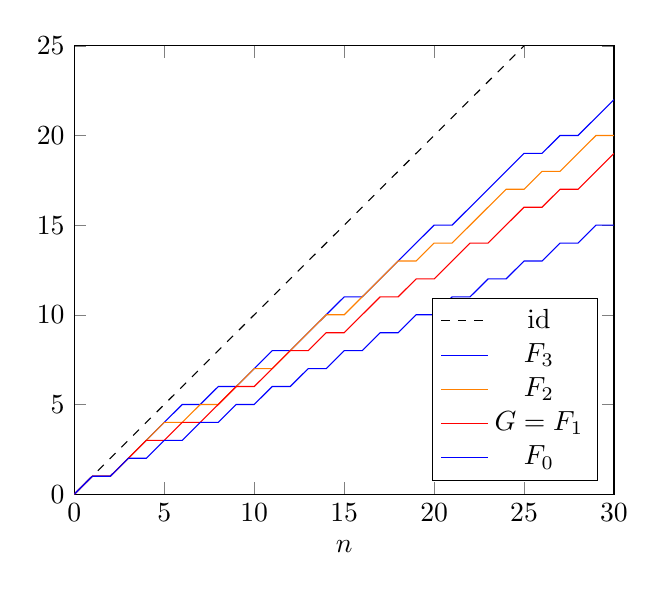
\begin{tikzpicture}[scale=1]
  \begin{axis}[
    xmin=0,xmax=30,ymin=0,ymax=25,samples=31,
    xtick = {0,5,...,30},
    ytick = {0,5,...,30},
    xlabel=$n$, legend pos=south east
  ]

 \addplot+[mark=.,color=black,style=dashed,domain=0:30] {x};
 \addlegendentry{id}
    \addplot [mark=.,color=blue] coordinates {
(0, 0) (1, 1) (2, 1) (3, 2) (4, 3) (5, 4) (6, 5) (7, 5) (8, 6)
 (9, 6) (10, 7) (11, 8) (12, 8) (13, 9) (14, 10) (15, 11) (16, 11)
 (17, 12) (18, 13) (19, 14) (20, 15) (21, 15) (22, 16) (23, 17)
 (24, 18) (25, 19) (26, 19) (27, 20) (28, 20) (29, 21) (30, 22)};
 \addlegendentry{$F_3$}
    \addplot [mark=.,color=orange] coordinates {
(0, 0) (1, 1) (2, 1) (3, 2) (4, 3) (5, 4) (6, 4) (7, 5) (8, 5)
 (9, 6) (10, 7) (11, 7) (12, 8) (13, 9) (14, 10) (15, 10) (16, 11)
 (17, 12) (18, 13) (19, 13) (20, 14) (21, 14) (22, 15) (23, 16)
 (24, 17) (25, 17) (26, 18) (27, 18) (28, 19) (29, 20) (30, 20) };
 \addlegendentry{$F_2$}
 \addplot+[mark=.,domain=0:30,color=red]
 {floor((x+1) * 0.618033988749894903)};
 \addlegendentry{$G=F_1$}
 \addplot+[mark=.,domain=0:30] {ceil(x/2)};
 \addlegendentry{$F_0$}
 \end{axis}
\end{tikzpicture}

\vspace{0.5cm}

\innerblock{ Theorem (with Shuo Li, nov. 2023!): }
{$\forall k,\forall n, F_k(n) \le F_{k+1}(n)$}
}%block
%\note[targetoffsetx = 3cm, targetoffsety = -20cm,
%       angle = -30, connection, width=12cm]{\Large Nov~2023:~Proved! }


\block{Fibonacci-like Sequences}{

For any $k\ge 0$:

\vspace{1cm}

\innerblock{Definition: the $A_k$ sequences}{
\begin{equation*}
\begin{cases}
A^k_n = n+1 \hfill \text{when}\ n\le k \\
A^k_{n+1} = A^k_{n} + A^k_{n-k} \hspace{5cm} \text{when}\ n+1 > k
\end{cases}
\end{equation*}
}

\vspace{1cm}

\begin{itemize}
\item $A^0$ : 1  2  4  8  16  32  64  128  256 $\ldots$
\item $A^1$ : 1  2  3  5  8  13  21  34  55  89 $\ldots$ (Fibonacci)
\item $A^2$ : 1  2  3  4  6  9  13  19  28  41 $\ldots$ (Narayana's Cows)
\item $A^3$ : 1  2  3  4  5  7  10  14  19  26 $\ldots$
\end{itemize}

\vspace{1cm}

\innerblock{Theorem:}{$\forall k, \forall n, F_k(A^k_n) = A^k_{n-1}$}

}%block

\block{Numerical Systems}{

\newcommand{\Arest}{\ensuremath{\Sigma A^k_i}}

\innerblock{Theorem (Zeckendorf):}{
Let $k\ge 0$. All $n\ge 0$ has a unique canonical decomposition
  $\Arest$ (i.e. with indices $i$ apart by at least $k+1$).
}

\vspace{1cm}

\innerblock{Theorem:}{
The function $F_k$ shifts down the indices of canonical
decompositions: $F_k(\Arest) = \Sigma A^k_{i-1}$ (with here $0-1 = 0$).
}

\vspace{1cm}

For instance for $k=2$ and $n=18$ :
\begin{itemize}
\item $18 = A^2_0 + A^2_3 + A^2_6 = 1 + 4 + 13$
\item $F_3(18) = A^2_0 + A^2_2 + A^2_5 = 1 + 3 + 9 = 13$
\item $1+3+9$ isn't canonical, renormalization possible
\end{itemize}

\vspace{1cm}

\innerblock{Theorem:}{
$F_k(n)=F_k(n+1)$ whenever $A^k_0=1$ is in the decomposition of $n$
  (we say $n$ has rank 0).
}

}%block


\column{.33}%CENTRE

\block{G as a Rational Tree}{

Let's repeat this branch pattern:

\vspace{1cm}

\begin{tabular}{lclclclc}
T & = & \hspace{-1cm}
\begin{tikzpicture}[grow'=up, level distance=2cm]
\Tree
     [.$\circ$ T
        [.$\circ$ [.T ]]]
\end{tikzpicture}
& = & \hspace{-1cm}
\begin{tikzpicture}[grow'=up, level distance=2cm]
\Tree
     [.$\circ$
       [.$\circ$ T
          [.$\circ$ [.T ]]]
       [.$\circ$ [.$\circ$ T
          [.$\circ$ [.T ]]]]]
\end{tikzpicture}
& = & \hspace{-1cm}
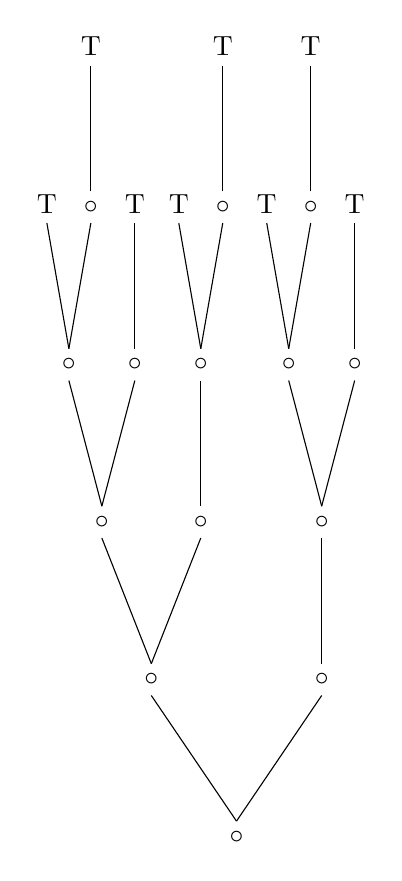
\begin{tikzpicture}[grow'=up, level distance=2cm]
\Tree
     [.$\circ$
       [.$\circ$ [.$\circ$ [.$\circ$ T
                                     [.$\circ$ T ] ]
               [.$\circ$ [.T ]]]
           [.$\circ$ [.$\circ$ T
                                           [.$\circ$ T ]]]]
       [.$\circ$ [.$\circ$ [.$\circ$ T
                                     [.$\circ$ T ]]
               [.$\circ$ T ]]]]
\end{tikzpicture}
& \hspace{-3cm} = $\ldots$

\end{tabular}

\vspace{1cm}

Now, with an ad-hoc trunk and node numbered via BFS:

\vspace{1cm}

\begin{tikzpicture}[grow'=up,level distance=2.5cm]

\bigskip
\bigskip

\Tree
 [.1 [.2 [.3
       [.4 [.6 [.9 [.14 22 23 ] [.15 24 ] ]
               [.10 [.16 25 26 ]]]
           [.7 [.11 [.17 27 28 ] [.18 29 ]]]]
       [.5 [.8 [.12 [.19 30 31 ] [.20 32 ]]
               [.13 [.21 33 34 ]]]]]]]
\end{tikzpicture}

\vspace{1cm}

\innerblock{Theorem:}{For any node $n>1$, its ancestor is $G(n)$. }

\vspace{1cm}

\innerblock{Exercise:}{ Which trees correspond to functions $F_k$ ? }

}%block

\block{Linear Equivalents}{

Let $\tau_k$ be the positive root of $X^{k+1}+X-1$. It is hence
algebraic, and irrational except for $k=0$.

\vspace{0.5cm}

\innerblock{Theorem:}{
For all $k\ge$, when $n\to\infty$ we have $F_k(n) = \tau_k.n + o(n)$
}

\vspace{0.5cm}
More precisely:
\vspace{0.5cm}

\coloredbox{
\begin{itemize}
\item $F_0(n) = \lfloor (n+1)/2 \rfloor = \lceil n/2 \rceil$
\end{itemize}}
And $A^0_n = 2^n$ and we retrieve the base-2 decomposition !

\vspace{0.5cm}

\coloredbox{
\begin{itemize}
\item $F_1(n) = G(n) = \lfloor \tau_1.(n+1) \rfloor$
\end{itemize}}
Here $\tau_1=1/\phi=\phi-1 \approx 0.618...$

\vspace{0.5cm}

\coloredbox{
\begin{itemize}
\item $F_2(n) - \lfloor \tau_2.n \rfloor \in \{0,1\}$
\end{itemize}}
Here $\tau_2 \approx 0.6823...$, inverse of Pisot number $P_3$. \\
With $\delta(n) = F_2(n) - \tau_2.n$, plotting $(\delta(i),\delta(F_2(i)))$
 leads to this Rauzy fractal !

\includegraphics[width=\linewidth]{fractal.png}

\vspace{0.5cm}

\coloredbox{
\begin{itemize}
\item $F_3(n) - \lfloor \tau_3.n \rfloor \in \{-1,0,1,2\}$
\end{itemize}}
Here $\tau_3 \approx 0.7244...$, inverse of Pisot number $Q_3$.

\vspace{0.5cm}

\coloredbox{
\begin{itemize}
\item After $k\ge 4$, $F_k(n)-\tau_k.n = o(n)$ but not bounded.
\end{itemize}}
Note: $\tau_4$ is the inverse of the Plastic number (smallest Pisot),
then $\tau_k$ for $k\ge 5$ is above any Pisot inverses.


}%block

\column{.33}%DROITE

\block{Morphic Words}{

We take $\mathcal{A}=\{0..k\}$ as alphabet.

\hspace{1cm}

\innerblock{Definition: the substitutions $\sigma_k$}{
\begin{equation*}
\begin{cases}
\mathcal{A} \to \mathcal{A}^* \\
\sigma_k(n) = (n+1) \hspace{7cm} \text{for}\ n<k \\
\sigma_k(k) = k.0
\end{cases}
\end{equation*}
}

\hspace{1cm}

\innerblock{Definition: the morphic words $m_k$}{

The substition $\sigma_k$ is prolongeable at k. It hence admits
an infinite word $m_k$ (called \emph{morphic}) as fixed point:

$$m_k = \lim_{n\to\infty} \sigma_k^n(k) = \sigma_k(m_k) $$
}

\hspace{1cm}

For instance:
\begin{itemize}
\item $m_1$ is the Fibonacci word (with inversed letters)
\item $m_2 = 20122020120122012202...$
\end{itemize}

\hspace{1cm}

\innerblock{Theorem:}{
$m_k$ is also the limit of its finite prefixes $M_{k,n}$ defined as:
\begin{equation*}
\begin{cases}
M_{k,n} = k.0...(n-1) \hfill \text{for}\ n\le k \\
M_{k,n+1} = M_{k,n}.M_{k,n-k} \hspace{5cm} \text{for}\ n+1 > k
\end{cases}
\end{equation*}

Also note that $|M_{k,n}| = A^k_n$
}

\hspace{1cm}

\innerblock{Theorem: linear complexity}{
The subword complexity of $m_k$ (i.e. its number of distinct factors of
size $p$) is $p \mapsto k.p+1$.
}

\hspace{1cm}

Lien avec $f_k$ :

La $n$-ième lettre $(m_k)_n$ du mot infini $m_k$ est le rang de la
$k$-decomposition de $n$ (ou $k$ si ce rang est plus de $k$).

En particulier cette lettre est 0 si $f_k(n)=f_k(n+1)$

En cumulant : le nombre de 0 dans $m_k$ entre 0 et $n$ est $n-f_k(n)$.

Plus généralement, compter les lettres au dessus de $p$ donne
$f_k^{(p)}$. En particulier le nombre de $k$ est $f_k^{(k)}$.

}%block

\block{Coq formalization}{
\begin{itemize}
\item Already $90\%$ of this poster defined and proved in Coq:
TODO URL %\url{https://github.com/letouzey/hofstadter_g}

\item Nearly 20\,000 lines of Coq formalization

\item Matrix (e.g. Vandermonde), polynoms, etc

\end{itemize}
}%block

\block{Thanks!}{

A big thanks to P.A. Melliès, W. Steiner, Y. Hu, S. Li

}%block

\block{References}{

TODO: Hofstadter, Fogg, Saari

}%block

\end{columns}

\end{document}
